\chapter{实验结果}
\label{chapter08}
{\em 本节给出所提出的基于归结的遗忘计算的实验结果,并分析实验结果。第\ref{chapter04}章提出的算法\ref{alg:compute:forgetting:by:Resolution}用Prolog语言实现,并在Linux服务器上进行了实验,该服务器是具有8个Intel核和32GB内存的i7CPU,其锁频和主频分别为4770 K和3.50 GHz。每次计算的时间限制到1200秒以内。
	实验分为两个部分:(1) 在随机数据集和标准数据集上的遗忘;(2) 在随机数据集上命题逻辑公式和$\CTL$公式的SNC计算。
	所有的实验数据和实验结果都可以从网上获取\footnote{ \url{https://github.com/fengrenyan/forgetting-in-CTL/tree/main/Appendix}}。
	
	此外,在这部分3-CNF公式$\varphi$的长度(记为$|\varphi|$)表示$\varphi$中子句的个数。}


\section{算法实现}


\section{遗忘实验分析}
这部分的实验数据分为两组:一组来源于标准数据集,一组是随机生成的数据。
标准数据集来源于$\CTL$-RP~\footnote{\url{https://sourceforge.net/projects/ctlrp/}}。但是由于数据集里的大部分公式是不可满足的,这种情形下遗忘的结果总是为$\bot$。因此,这里对数据集进行了简单的处理:从标准数据集里抽取了“sample01”文件中的s001.ctl、s002.ctl、s003.ctl和s004.ctl文件,并从这些公式里取前面的两个子公式的合取构成新的公式,分别称为s001、s002、s003和s004。此外,从s001.ctl中取前三个子公式的合取构成新的公式s001-3。

计算{\CTL-forget}$(\varphi, V)$所使用的CPU时间(单位:秒(s),不指出时也默认为秒)如表\ref{chapter04:tab:sample}所示,其中$\varphi\in \{s001,s002,s003,s004,s001$-$3\}$,$|V|\in \{1,2,3,4\}$。
从中可以看出公式长度越长、被遗忘的原子命题个数越多,则计算所需要的时间越长。

\begin{table}%[width=.9\linewidth,cols=4,pos=h]
	\small
	\centering
	\caption{计算 {\CTL-forget}$(\varphi, V)$所使用的CPU时间(单位:秒(s))}\label{chapter04:tab:sample}
	\setlength{\tabcolsep}{5mm}{
		\begin{tabular}{l|llll}%{@{} L|LLLL@{} }
			\toprule
			\diagbox[width=6em]{$\varphi$}{$|V|$}&
			1        & 2       & 3        & 4   \\
			\midrule
			\texttt{s001}         & 0.0505 & 0.1053 & 0.2259 & 0.3680 \\ 
			\texttt{s002}         & 0.3645          & 1.0416          & 5.6372          & 10.0184          \\ 
			\texttt{s003}         & 97.5341          & 71.5396          & 190.1157          & 423.5793          \\ 
			\texttt{s004}         & 77.5086          & 77.4246          & 101.1284          & 118.7461          \\ 
			\texttt{s001-3} & 681.2883   & 613.1859 & 1617.047 & 2356.949 \\
			\bottomrule
	\end{tabular}}
\end{table}

除了上述标准数据集中的公式,我们也做了具有以下形式的公式的遗忘实验:
$$\varphi=\varphi_1 \wedge \ALL\NEXT \varphi_2 \wedge \EXIST\NEXT \varphi_3$$
其中$\varphi_i$($i=1,2,3$)是随机产生的定义在原子命题集合$\Ha$上的3-CNF公式,且$|\varphi_1| = |\varphi_2| =|\varphi_3|$、$|\Ha|=4$。
这里做了六组计算$\CTLforget(\varphi,V)$的实验,即$|\varphi_i| \in \{12,16\}$和$|V|\in \{1,2,3\}$的组合,每一组有二十个公式。

$|\varphi_i|=12$时的实验结果如图\ref{chapter04:fig:for12}所示,图\ref{chapter04:fig:for12}(a) 展示了计算遗忘所需要的时间,图\ref{chapter04:fig:for12}(b)展示了在计算过程“移除原子命题”后$\CTLsnf$子句的个数。其中$x$轴表示第几个公式,$y$轴分别表示时间和数量。
从图\ref{chapter04:fig:for12}里面可以看出,需要遗忘的原子命题个数越多,所用时间越长且在“移除原子命题”后剩余的$\CTLsnf$子句的个数越少。
当$|\varphi_i|=16$时的实验结果如图\ref{chapter04:fig:for16}所示,其与$|\varphi_i|=12$时有相似的结果。

\begin{figure*}[!htb]
	\centering
	\subfigure[计算遗忘需要的CUP时间]{
		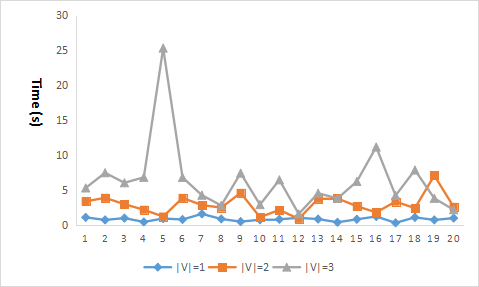
\includegraphics[width=7cm]{chapter04/time_4_12.png}
	}
	\subfigure[$\CTLsnf$子句的个数]{
		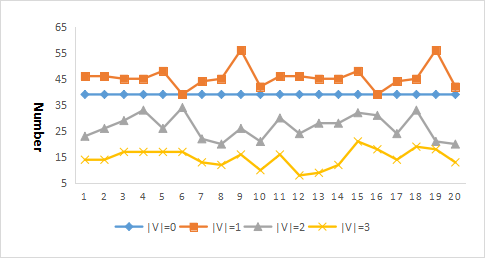
\includegraphics[width=7cm]{chapter04/number-4-12.png}
	}
	\caption{计算{\CTL-forget}$(\varphi, V)$使用的时间和在“移除原子命题”步骤后$\CTLsnf$子句的个数,其中$\varphi_i=12$。}
	\label{chapter04:fig:for12}
\end{figure*}

\begin{figure*}[!htb]
	\centering
	\subfigure[计算遗忘需要的CUP时间]{
		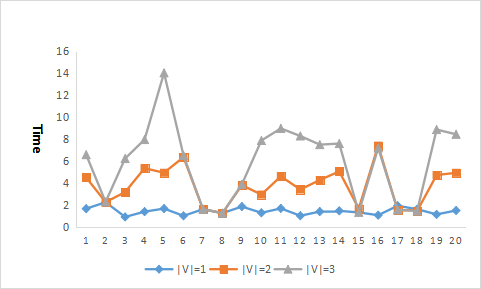
\includegraphics[width=7cm]{chapter04/time_4_16.png}
	}
	\subfigure[$\CTLsnf$子句的个数]{
		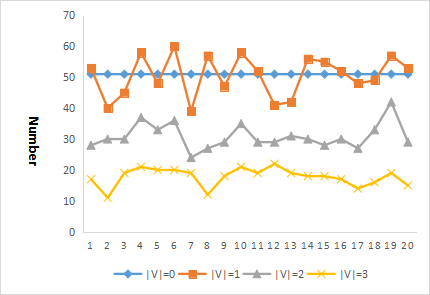
\includegraphics[width=7cm]{chapter04/number-4-16.png}
	}
	\caption{计算{\CTL-forget}$(\varphi, V)$使用的时间和在“移除原子命题”步骤后$\CTLsnf$子句的个数,其中$\varphi_i=16$。}
	\label{chapter04:fig:for16}
\end{figure*}

\section{SNC计算结果分析}
这部分实验分析使用基于遗忘的方法计算$\CTL$公式的SNC,分为两组实验:分别计算经典命题公式和$\CTL$公式的SNC,即:计算$q$在$V$和$\varphi \wedge q$上的SNC($\CTLforget(\varphi\wedge q, \Var(\varphi)-V \cup \{q\})$),其中$V\subseteq \Var(\varphi)$、$q\in \Var(\varphi\wedge q)-V$。
这些公式$\varphi$都是随机生成的定义在原子命题集合$\Ha$上的公式、$V$也是在计算过程中随机生成的、$q\not \in \Var(\varphi)$是一个固定的原子命题且$|\Ha|=50$。

首先测试随机3-CNF命题公式。令$|V|$的取值范围为$\{5,10,\dots, 40,45\}$,3-CNF公式的子句个数$nc$范围为$\{10,15,\dots, 45,50\}$。
在每种情形当中,计算20个随机实例$(\varphi,q,V)$:$\varphi$为$\Ha$上的公式,且$V\subseteq \Var(\varphi)$。
计算SNC的平均CPU时间如图\ref{chapter04:fig:ProTime}所示。

\begin{figure*}[!htb]
	\centering
	\subfigure[平均CPU时间(s)]{
		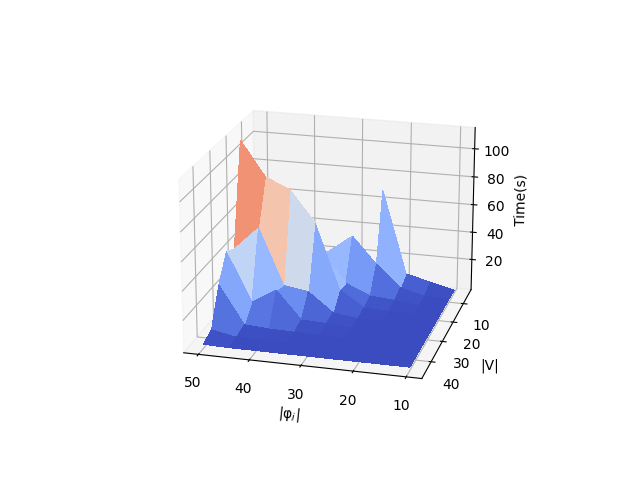
\includegraphics[width=7.5cm]{chapter04/PRototalAveTime.png}
	}
	\subfigure[$|V|=25$时所使用CPU时间箱线图 % and $|\varphi|~\in~ \{10, 15,\dots, 50\}$
	]{
		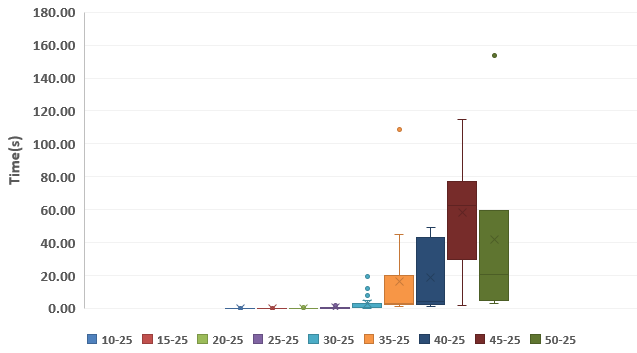
\includegraphics[width=7cm]{chapter04/ProBox(10-50)_25.png}
	}
	\caption{%The performances of computing SNC in PL.
		计算3-CNF公式SNC的CPU时间}
	\label{chapter04:fig:ProTime}
\end{figure*}


从图\ref{chapter04:fig:ProTime}(a)可看出,随着$|\varphi|$增大或$|V|$的减小时间消耗越大。
直观地说,越大的$|\varphi|$或者越小的$|V|$意味着$\CTLforget(\varphi, \overline{V})$更难计算。
这与上一小节中的结论相符合。
图\ref{chapter04:fig:ProTime}(b)展示了当$|V|= 25$、$nc\in \{10,15,\dots, 45, 50\}$时20个随机实例的箱线图。
这同样证明了$nc$越大SNC越难计算。


其次,测试具有如下形式的$\CTL$公式的SNC的计算:
$$\varphi_1 \wedge \ALL \NEXT \varphi_2 \wedge \EXIST\NEXT \varphi_3$$
其中$\varphi_i$($i=1,2,3$)为随机产生的定义在$\Ha$上的3-CNF公式,且满足$|\varphi_1|=|\varphi_2|=|\varphi_3|$。
在这种情形下,每个实例$(\varphi, q, V)$是随机产生的,其中$\varphi=\varphi_1 \wedge \ALL \NEXT \varphi_2 \wedge \EXIST\NEXT \varphi_3$、$V\subseteq \Var(\varphi)$、$|\varphi|\in \{5,6,\dots, 13,14\}$、且$|V|\in \{15,16,\dots, 23,24\}$。
值得注意的是在实例$(\varphi, q, V)$中,$q$可能没有在$V$和$\varphi\wedge q$上的SNC。

图\ref{chapter04:fig:CtlTime}(a)展示了每种情形计算40个实例的SNC的平均CPU时间。与命题公式的情形相似,越大的$|\varphi|$或者越小的$|V|$意味着$\CTLforget(\varphi, \overline{V})$更难计算。
此外,图\ref{chapter04:fig:CtlTime}(b)展示了每种情形下40个实例中SNC存在的占比,即:$|\varphi|$越小或者$|V|$越小则SNC存在的占比越大。特别地,当$|\varphi_i|=5$且$|V|=16$时,SNC存在的占比为80\%。



\begin{figure*}[!htb]
	\centering
	\subfigure[平均CPU时间(s)]{
		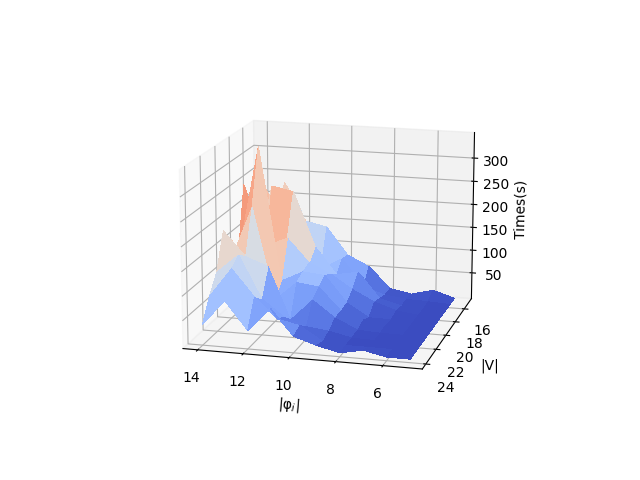
\includegraphics[width=7cm]{chapter04/totalAveTime.png}
	}
	\subfigure[存在SNC的公式占比(\%)]{
		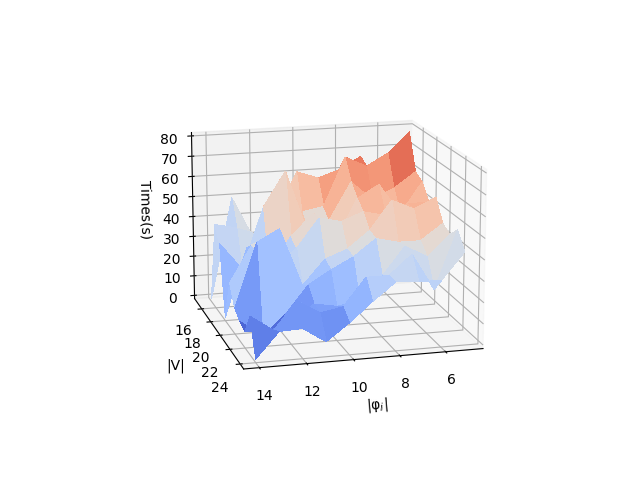
\includegraphics[width=7cm]{chapter04/numPercent.png}
	}
	\caption{计算$\CTL$SNC的平均时间和存在SNC的公式占比.}
	\label{chapter04:fig:CtlTime}
\end{figure*}

综上所述,算法\ref{alg:compute:forgetting:by:Resolution}大多数情况下能计算出SNC(WSC),且当需要遗忘的原子个数很少或公式长度较小的时候计算效率很高。

\section{本章小结}\label{sec:chapter06-conclusion}

本章从两个角度来评估第\ref{chapter04}章提出的算法的实现。从标准数据集中获取的公式和随机产生的公式下遗忘的计算对需要遗忘的原子命题的个数和公式的长度都很敏感:要遗忘的原子命题个数越多或公式越长,计算效率越低。
此外,关于计算SNC的实验表明本文提出的算法在实验给出的数据集中的大部分情况下是能计算出SNC的。三维图和箱线图都表示计算SNC体现了跟计算遗忘一样的规律,这与SNC是由遗忘来计算是一致的。
